\section{Signal Model}
\label{sec:model}

% figure 1 should be revisit.
\begin{figure*}[t]
  \centerline{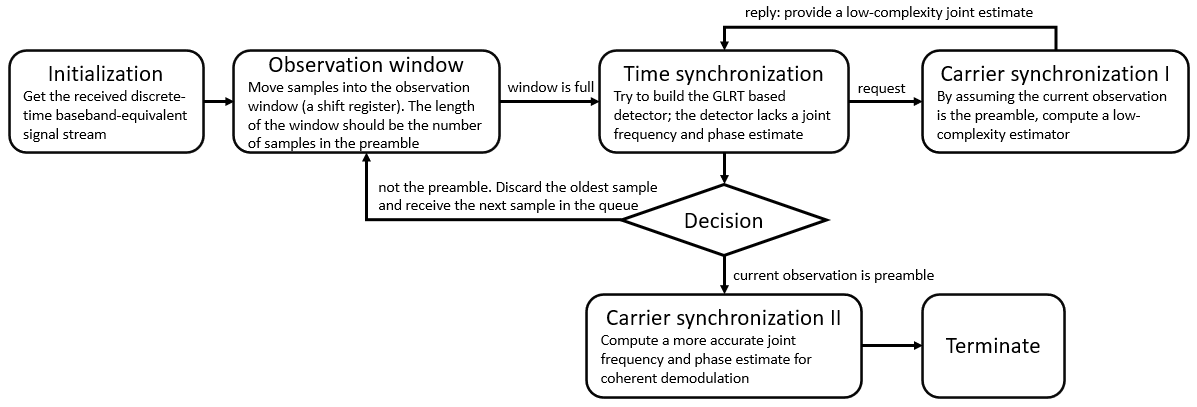
\includegraphics[width=6.5in]{signal_acquisition_chain.png}}
  \caption{Block diagram for analysis of the complete signal acquistion chain}
  \label{fig:sig_acquis_chain}
  \end{figure*}

The transmitted signal burst is assumed to include a refere\-nce signal that is known to the receiver.
Often such a reference sequence is prepended to the payload and is referred to as a preamble.
The problem addressed in this paper is to accurately estimate the start time of the preamble and 
to estimate carrier phase and frequency offset from this preamble.
Hence, the payload portion of the burst is not further considered.

The baseband-equivalent reference signal $s(t)$ is digitally modulated as

\begin{equation}
    \label{eq:l_ref_sig_analog}
    s(t) = \sum_{i=0}^{L_0-1} c_i g(t-iT),
  \end{equation}
where $T$ denotes the symbol period and $g(t)$ provides pulse shaping. $\{c_i\}_{i=0}^{L_{0}-1}$ is the known symbol sequence
between tran-smitter and receiver, where $L_0$ denotes the number of symbols. It is common to assume the symbols 
$c_i$ have good autocorrelation properties to render coherent processing effective.

At the receiver side, the received baseband equivalent signal stream are given by

\begin{equation}
    \label{eq:rec_sig_analog}
    r(t) = s(t-\tau) \cdot Ae^{j \phi} e^{j2\pi f_d t} + w(t).
  \end{equation}
where $\tau$ denotes the delay (the start time) of received reference signal in the stream. $A$, $\phi$, $f_d$ 
are the carrier amplitude, phase, and frequency offset, respectively. These are the parameters to be estimated
for signal acquisition in this paper. The complex, additive white Gaussian noise is denoted $w(t)$.

Our algorithms are discussed in discrete-time; sampling the received signal $r(t)$ at a rate of $M$ samples per symbol,
i.e., the sampling frequency $f_s=\frac{1}{T_s}=\frac{M}{T}$, yields 

\begin{equation}
    \begin{aligned}
      \label{eq:model}
      r_n = s_{n-p}^{(\Delta p)}Ae^{j\phi}e^{j2\pi\delta n}+w_{n},
    \end{aligned}
  \end{equation}
where, the continuous-time delay $\tau$ is decomposed into $\tau=pT_s+\Delta p$ with $pTs$ integer multiples of sample period and 
the fractional delay $\Delta p$ satisfying $-Ts/2 {<} \Delta p {\leq} T_s/2$. Thus, $\Delta p$ is negatively correlated with
the sampling frequency. Moreover, the sampled received reference sequence, including the effect of fractional delay, is

\begin{equation}
  \label{eq:l_ref_sig_discrete}
  s_n^{(\Delta p)} = \sum_{i=0}^{L_0-1} c_i g(nTs-iT-\Delta p) \quad \text{for}~n=0,\ldots,N-1,
\end{equation}
where $N=ML_0$ is the number of samples in the preamble. When $\Delta p=0$, $s_n^{(\Delta p)}$ is simply denoted as $s_n$.

In~\eqref{eq:model}, $\delta$ denotes the normalized frequency offset $\delta=f_dT_s$. This normalized offset
will be estimated and is of relevance for the demodulator. However, for comparing estimation accuracy for different
sampling rates we will normalize with respect to the symbol period $T$. For example, the simulation results for frequency estimate 
in Section~\ref{sec:simulations} show the mean-squared error of $\frac{T}{T_s}\delta=M\delta$.
Besides that, $E_s/N_0$ represents the ratio of signal energy to noise power spectral density (SNR).
Specifically, $E_s$ is the averaged symbol energy of the received signal over the length of the preamble.

% estension to reviewer 3, comment 3
The rest of paper is seperated into two main sections. The first main section (Section~\ref{sec:detection} and~\ref{sec:freq_est}) focus on analyzing the complete
signal acquisition chain, which basically includes delay estimation of the preamble (detection) and
carrier synchronization. The process in general is shown in Figure~\ref{fig:sig_acquis_chain}.
The simulation section (Section~\ref{sec:simulations}) then illustrates the performance of the proposed algorithm in first section.
The second section (Section~\ref{sec:real_implementation}) moves attention on implementing the algorithm 
on software-defined radio (SDR). Some steps (equations) of the algorithm in the first section are computed more efficiently to achieve the best throughput.

